\documentclass[11pt,a4paper,openright]{book}
%\documentclass[11pt,a4paper,openany]{book}
\usepackage[dvipdfmx]{graphicx}
%\usepackage{graphicx}
%\usepackage{float}
%\usepackage{otf}
\usepackage{multirow}
\usepackage{lscape}
\usepackage{amsmath}
\pagestyle{headings}
%\usepackage{citesort}

%\setlength{\topmargin}{10mm} %上マージン 10mm
\addtolength{\topmargin}{-5mm} % 標準のマージン(1inch)を引く
\addtolength{\textheight}{12mm} %本文の長さ (縦) 297-(10+27)= 250
\usepackage{layouts}

\newcommand\DocLength[1]{%
  The value for \texttt{#1} is \printinunitsof{pt}\prntlen{\csname#1\endcsname}\par}

%\addtolength{\oddsidemargin}{-20mm} 
\addtolength{\marginparwidth}{-106pt} 
\addtolength{\marginparsep}{-7pt} 
\addtolength{\evensidemargin}{-70pt} 
\addtolength{\oddsidemargin}{-22pt} 
\addtolength{\evensidemargin}{-1in} 
\addtolength{\oddsidemargin}{-1in} 
\addtolength{\evensidemargin}{24mm} 
\addtolength{\oddsidemargin}{36mm} 
% 奇数ページ 左マージン 20mm
%\addtolength{\oddsidemargin}{-1in} % 奇数ページ 標準のマージン(1inch)を引く
%\setlength{\oddsidemargin}{10mm} % 偶数ページ 左マージン 10mm
%\setlength{\evensidemargin}{10mm} % 偶数ページ 左マージン 10mm
%\setlength{\evensidemargin}{30mm} % 偶数ページ 左マージン 10mm
%\addtolength{\evensidemargin}{-1in} % 偶数ページ 標準のマージン(1inch)を引く
\setlength{\textwidth}{150mm} %本文の長さ(横) 210 -(20+20) = 170
\title{}
\begin{document}
\if0
\DocLength{evensidemargin}
\DocLength{oddsidemargin}
\DocLength{hoffset}
\DocLength{marginparwidth}
\DocLength{marginparsep}
\fi
%\section{Beamline}

\subsection{BHD and T0}
The beam particles are kaon is confirmed by the TOF method using beamline hodoscope detector (BHD) and time-zero counter (T0) in the offline analysis.
The T0 is located immediately downstream of the AC.
The BHD is located between the D5 and D4 magnets, approximately 7.7m upstream of T0, i.e. the flight length is 7.7m.

The T0 is a 5-segment plastic scintillation counter array 160mm (high) $\times$ 32mm (width) $\times$ 10mm (thick), with an effective area of 160mm $\times$ 160mm.
The T0 is installed rotated 45 degrees with respect to the beam direction as the beam is horizontally spread at the T0.
A counter uses the Saint-Gobain BC420 scintillator and attached readout which is 3/4 inch Hamamatsu H6612B photomultipliers to both sides of the scintillator.

The BHD is a 20-segment plastic scintillation counter array 160mm (high) $\times$ 20mm (width) $\times$ 5mm (thick), with an effective area of 200mm (horizontal) $\times$ 160mm (vertical).
A counter uses the same photomultipliers as the T0 counter.
The BHD is installed at the most upstream of the beamline and the number of beams per spill is a few M ($\times 10^6$)events,
so the photomultipliers are attached high voltage booster to the last three dynodes to avoid gain drop due to high current by high rate beam.

\subsection{Beam line chamger}
\begin{figure}[htbp]
  \centering
  \begin{tabular}{ccc}
    \begin{minipage}{0.33\hsize}
      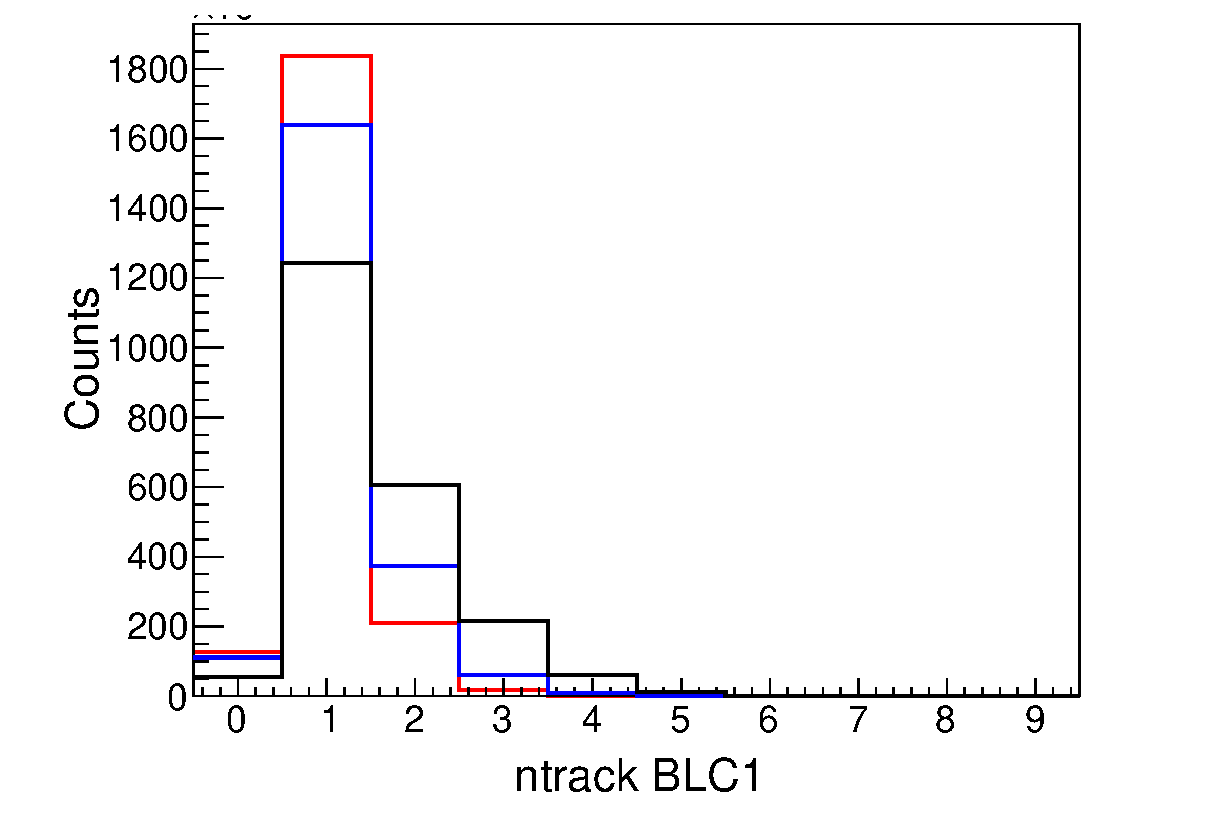
\includegraphics[width=4cm]{../pic/Run78/BL/nBLC1.eps}
    \end{minipage}
    \begin{minipage}{0.33\hsize}
      \includegraphics[width=4cm]{../pic/Run78/BL/BLC1_time.eps}
    \end{minipage}
    \begin{minipage}{0.33\hsize}
      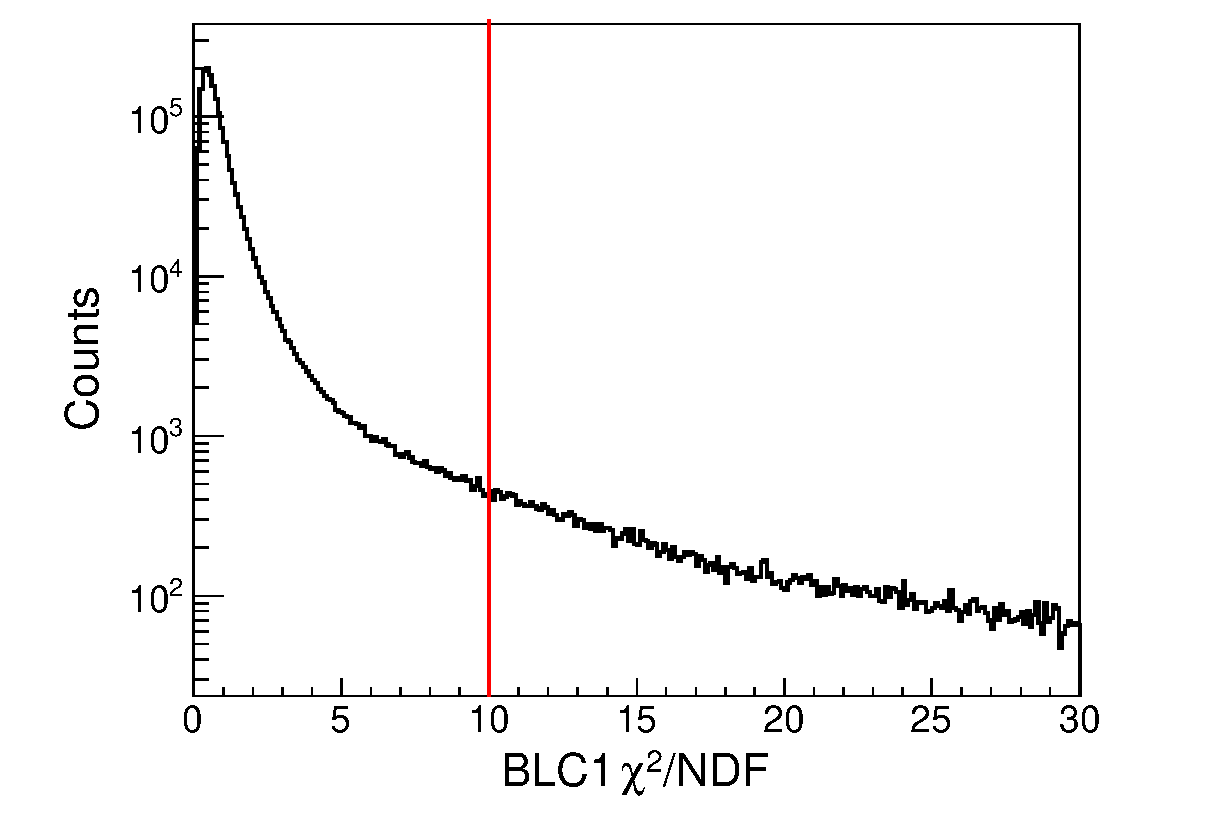
\includegraphics[width=4cm]{../pic/Run78/BL/BLC1_chi2.eps}
    \end{minipage}
  \end{tabular}
  
  \begin{tabular}{ccc}
    \begin{minipage}{0.33\hsize}
      \includegraphics[width=4cm]{../pic/Run78/BL/nBLC2.eps}
    \end{minipage}
    \begin{minipage}{0.33\hsize}
      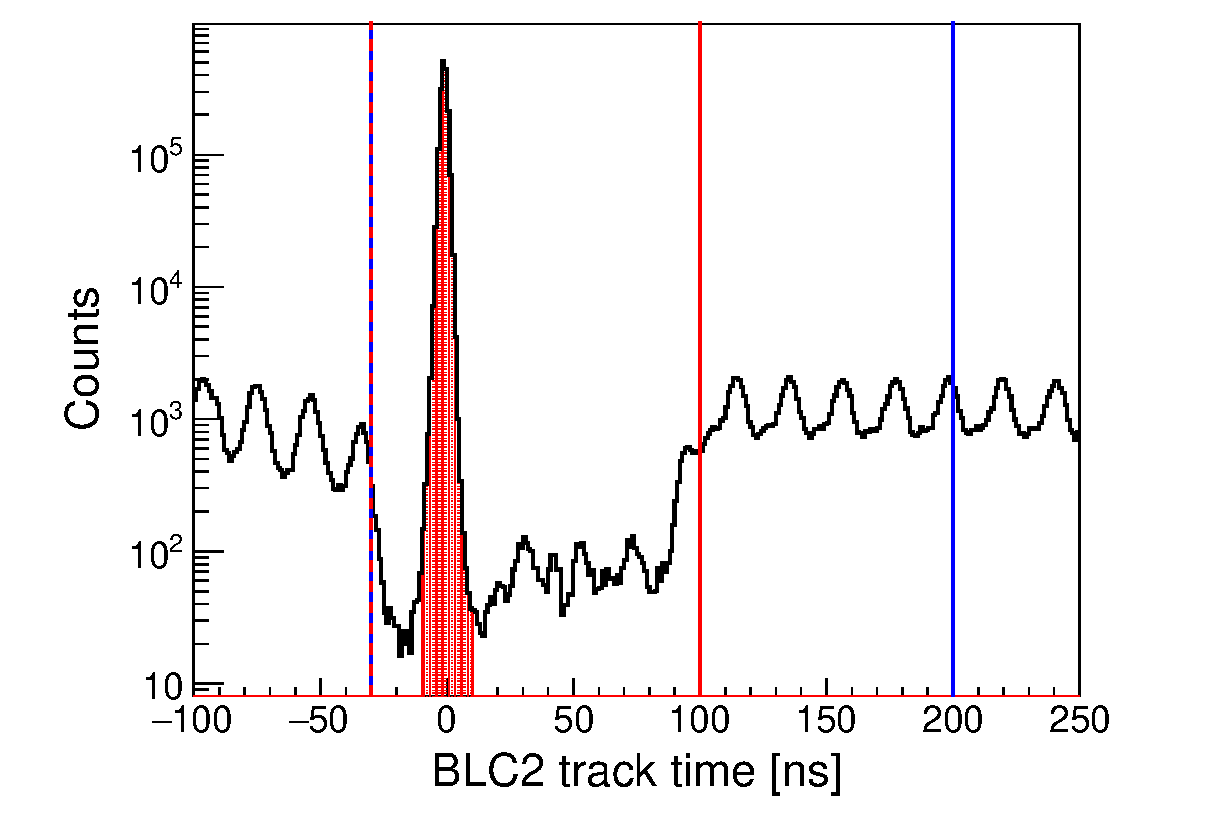
\includegraphics[width=4cm]{../pic/Run78/BL/BLC2_time.eps}
    \end{minipage}
    \begin{minipage}{0.33\hsize}
      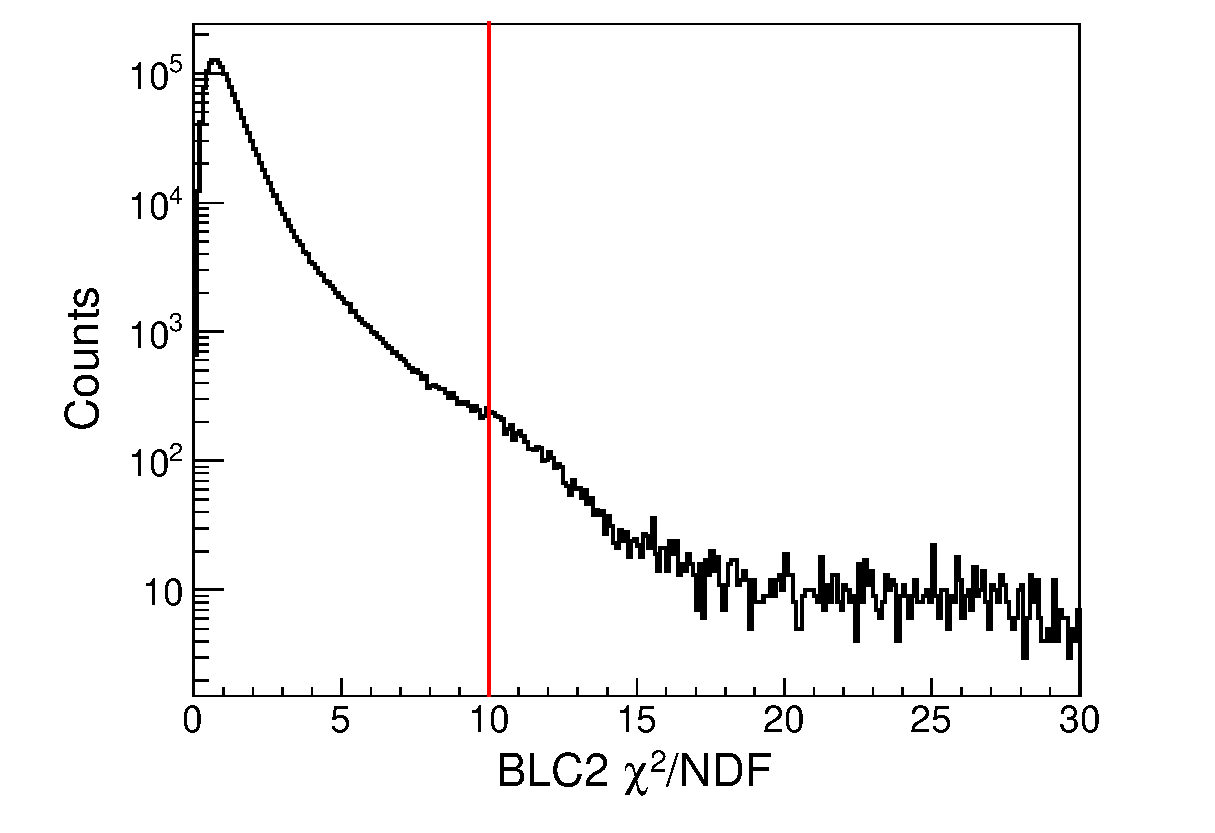
\includegraphics[width=4cm]{../pic/Run78/BL/BLC2_chi2.eps}
    \end{minipage}
  \end{tabular}
  
  \begin{tabular}{ccc}
    \begin{minipage}{0.33\hsize}
      \includegraphics[width=4cm]{../pic/Run78/BL/nBPC.eps}
    \end{minipage}
    \begin{minipage}{0.33\hsize}
      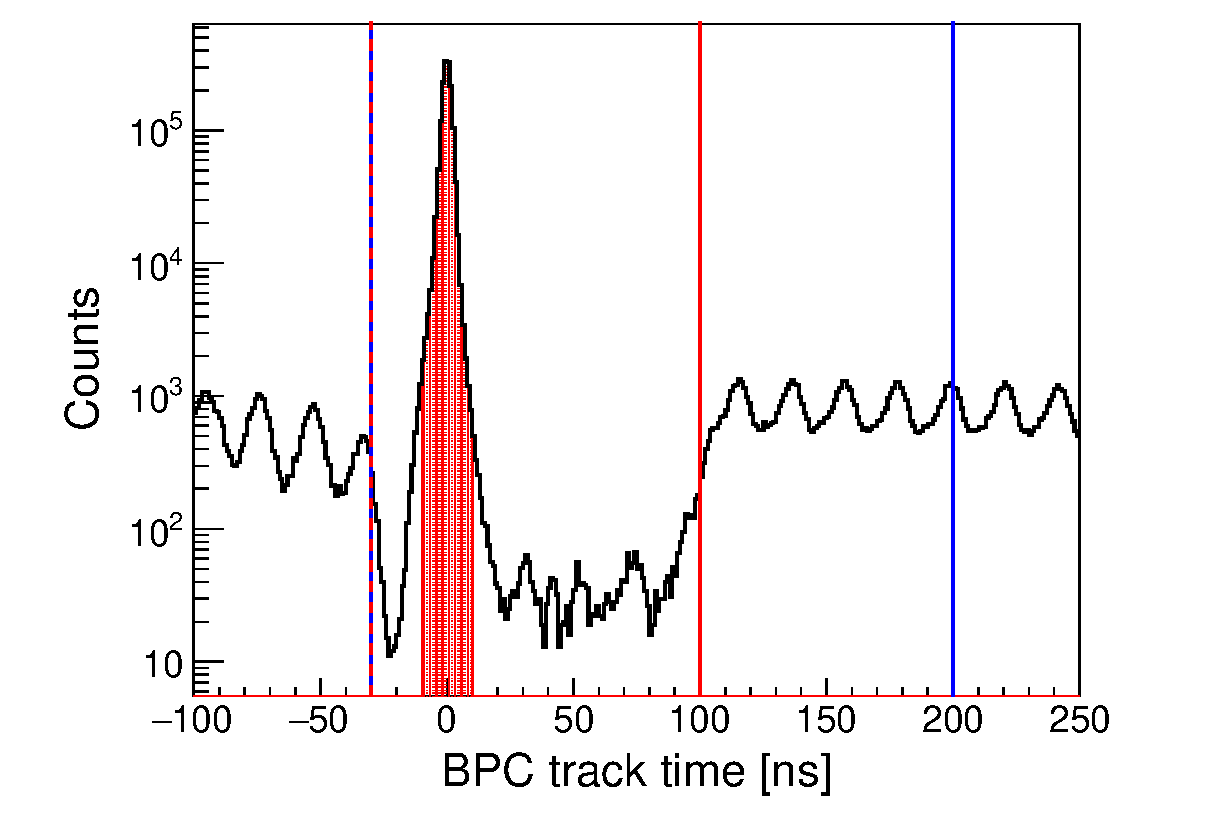
\includegraphics[width=4cm]{../pic/Run78/BL/BPC_time.eps}
    \end{minipage}
    \begin{minipage}{0.33\hsize}
      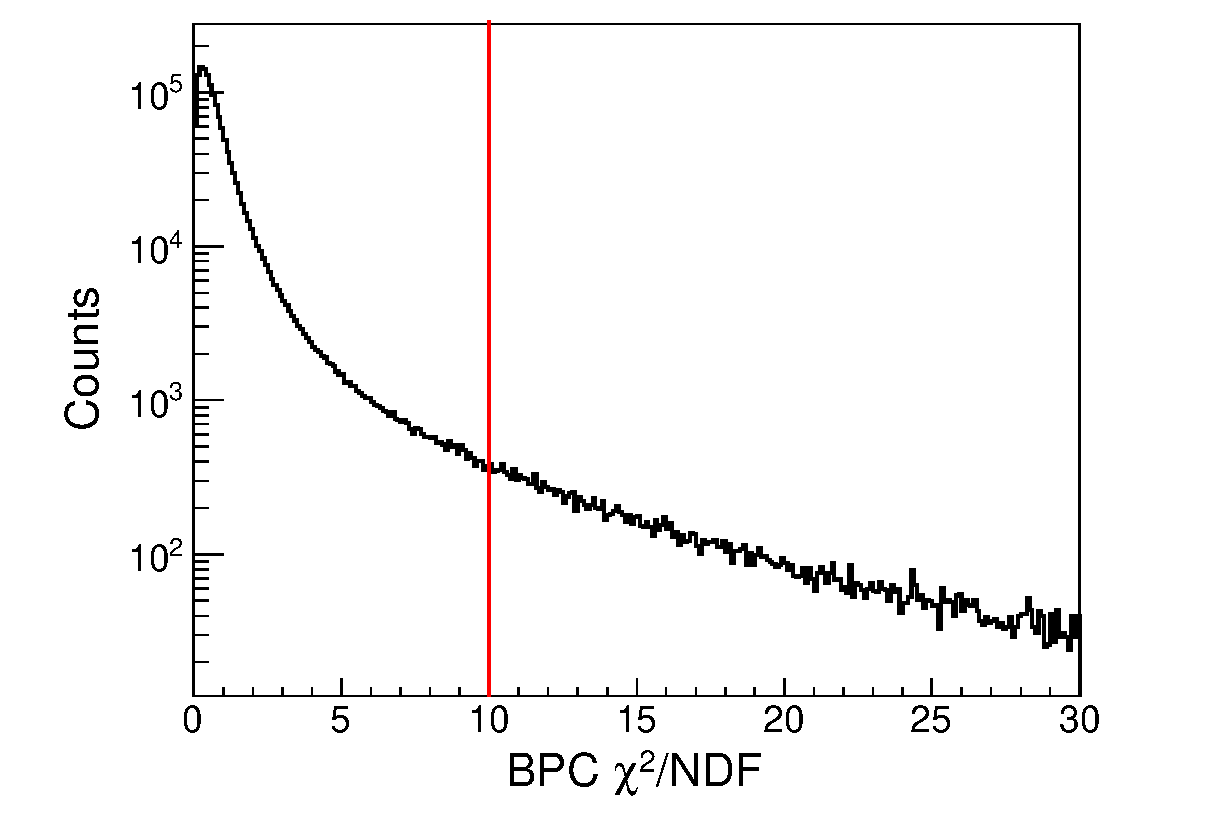
\includegraphics[width=4cm]{../pic/Run78/BL/BPC_chi2.eps}
    \end{minipage}
  \end{tabular}
  \caption{
    The left, the middle and the right figures show the number of tracks, track time and $\chi/NDF$, respectively.
    Color plots in the left figure indicate some time window.
    % Black, blue, red indicate all, $-30\sim200$[ns], $-30\sim100$[ns], respectively.
    The above, the middle and the down figures represent BLC1, BLC2 and BPC, respectively.
    The BPC was described after.
  }
  \label{fig:BLC_etc}
\end{figure}
BLC1 and BLC2 were installed upstream and downstream of the D5 magnet, respectively to measure beam momentum using the transfer matrix of the D5 magnet.
These are planer the type drift chamber whose drift length was calculated using the X-T map, which was the integration of drift time.
The track time of BLC was estimated from timing signals of pair plane due to constant drift length.
SX beam has RF-structure seems like the center figures of Fig\ref{fig:BLC_etc}, so we select synchronization about beam which indicates the red hatched region.
The left figures represent the number of tracks, in which black, blue, and red indicate time window of all, $-30\sim100$[ns], and $-30\sim200$[ns], respectively.
We select 1track events in red time window selection to keep statistics.
The right figures show $\chi^2/NDF$ distribution after 1track selection.
We accepted $\chi^2/NDF<10$ events as good track.



\chapter{$\Lambda p$ event analysis}
In Sec. \ref{sec-multin}, the contribution of the multi-nucleon absorption processes was evaluated by using the $\Lambda p$ event distribution in the $K\otimes {\rm CDH}^{2 hits}$ trigger data. Here, the $\Lambda p$-event selection and the normalization factors for an evaluation of the yields of the $\Lambda p$ events are described.
\section{Event selection}
In order to reconstruct a pair of $\Lambda p$, one $\pi^-$ and two protons were required to be detected with the CDS. Events with more than 3 tracks were discarded. The two protons were checked whether either of them can reconstruct $\Lambda$ with the $\pi^-$.  Figure \ref{fig-lpselection}(left) shows the correlation of the two $p\pi^-$ invariant masses with each proton. The distance of closest approaches (DCAs) between the beam track and the reconstructed $p\pi^-$ parent track to discriminate the proton from the $\Lambda$ decay and the $p_1\pi^-$ pair was defined to give shorter DCA than the $p_2\pi^-$ pair. Although the $p_1\pi^-$ pair is naively expected to be more likely to be $\Lambda$ origin, the $p_2\pi^-$ pairs also contains $\Lambda$s  as a horizontal line is seen in Fig. \ref{fig-lpselection}(left). Therefore, the $p\pi^-$ pair whose invariant mass was closer to the $\Lambda$ mass was selected as a $\Lambda$ candidate and filled in Figure \ref{fig-lpselection}(right). The $\Lambda$ and side-band regions are also defined in Figure \ref{fig-lpselection}(right). The signal-to-noise ratio at the $\Lambda$ peak was approximately 5. Figure \ref{fig-lpinvmm} shows $^3$He($K^-,\Lambda p)X$ missing-mass and $\Lambda p$ invariant-mass spectra compared with side-band events in $\Lambda$ selection.

\begin{figure}[]
\begin{center}
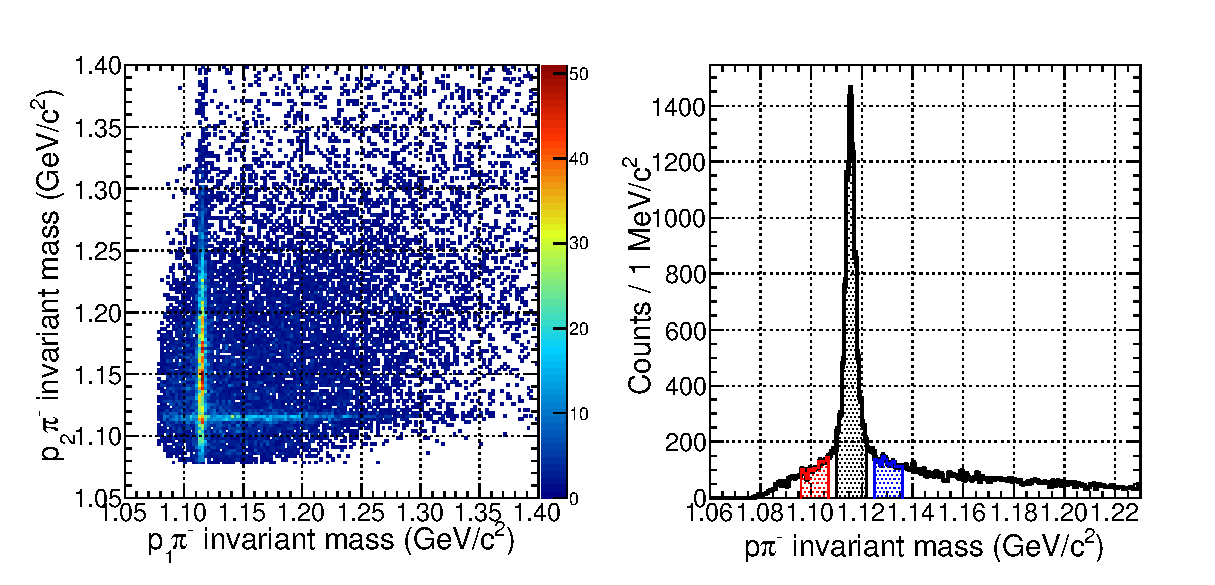
\includegraphics[width=\columnwidth]{./fig/lp_selection.eps}
\caption[Correlation of $p\pi^-$ invariant masses reconstructed with each proton in the $\pi^-pp$ events.]{(left) Correlation of $p\pi^-$ invariant masses reconstructed with each proton in the $\pi^-pp$ events. $p_1\pi^-$ has shorter DCA between the beam and reconstructed parent tracks than $p_2\pi^-$. (right) $p\pi^-$ invariant mass distribution in the $\pi^-pp$ events. The $p\pi^-$ pair whose invariant mass is closer to the $\Lambda$ mass is filled. The black hatched region represents $\Lambda$ selection, while blue and red hatches represent the side band regions.}
\label{fig-lpselection}
\end{center}
\end{figure}  

\begin{figure}[]
\begin{center}
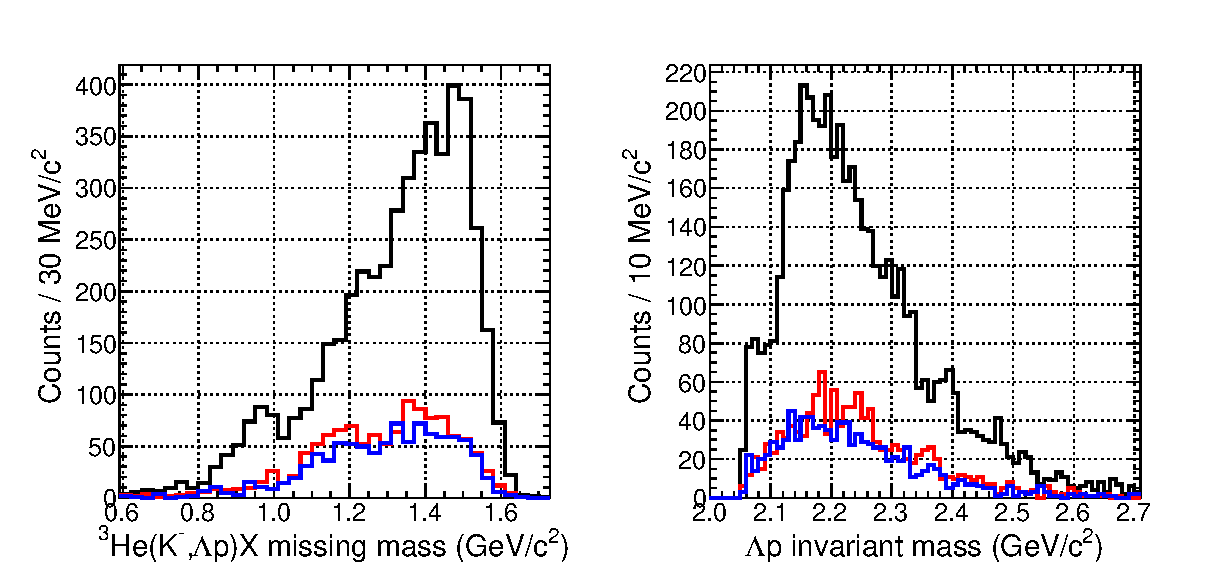
\includegraphics[width=\columnwidth]{./fig/lp_invmm.eps}
\caption[$^3$He($K^-,\Lambda p)X$ missing-mass and $\Lambda p$ invariant-mass spectra.]{(left) $^3$He($K^-,\Lambda p)X$ missing-mass and (right) $\Lambda p$ invariant-mass spectra. The blue and red histograms represent the side-band events in the $\Lambda$ selection as defined in Fig. \ref{fig-lpselection}.}
\label{fig-lpinvmm}
\end{center}
\end{figure}  

\section{Normalization}
The total cross-section of the $\Lambda p$ events can be expressed as,
\begin{eqnarray}
\sigma =\frac{1}{L}\cdot\frac{1}{\epsilon_{CDC}^3\cdot\epsilon_{PID}^3\cdot A'_{CDS}}\cdot\frac{1}{\epsilon'_{DAQ}\cdot\epsilon'_{trig}}\cdot N,
\end{eqnarray}
where $L$ and $\epsilon_{CDC}$ are the integrated luminosity and the CDC tracking efficiency, which are the same as those in Eq. \ref{eq-ncs}. $\epsilon_{PID}$ and $\epsilon'_{trig}$ are the efficiencies of the particle identification in the CDS and the $K\otimes CDH^{2 hits}$ trigger, which were assumed to be unity for the simplicity. $A'_{CDS}$ is the acceptance of the CDS to reconstruct three charged particles, $\pi^-pp$, evaluated by the simulation assuming phase-space uniform distribution of the multi-nucleon processes. $\epsilon'_{DAQ}$ is the live rate of the DAQ system with a consideration of the pre-scale factor of 7. These values are summarized in Table \ref{tab-lp}.

\begin{table}[]
\caption{Normalization factors for the $\Lambda p$ events.}
\begin{center}
\begin{tabular}{lc}
\hline\hline					
Luminosity $L$	($\mu$b$^{-1}$)	&	540					\\
$\epsilon_{CDC}$		&	0.96					\\
$\epsilon_{PID}$		&	1					\\
$\epsilon_{DAQ}'$		&	0.116					\\
$\epsilon_{trig}'$		&	1					\\
\hline\hline
\end{tabular}
\end{center}
\label{tab-lp}
\end{table}%


\section{$\Lambda pn$ final state}
It is worth mentioning that we can identify $\Lambda pn$ final state as a missing neutron peak in the $^3$He($K^-,\Lambda p)X$ missing-mass spectrum. If these events are attributed to NM2NA with a neutron spectator, we expect a corresponding peak around 2.8 GeV/$c^2$ in the $\Lambda p$ invariant-mass spectrum. No significant structure above 2.7 GeV/$c^2$ in Fig. \ref{fig-mmlpfit}(right) suggests that most of the $\Lambda pn$ events are attributed to 3NA. However, due to the limited statistics of the $\Lambda p n$ events, more detailed analysis cannot be achieved at present; we have obtained a few hundred $\Lambda p n$ events in the $^3$He$(K^-,\Lambda p)X$ missing-mass spectrum, in which only $\sim$ 10 events are available if we require the neutron to be detected with the NC. 

%\chapter{Run dependence}
\clearpage
\section{Kaon beam analysis}
\begin{figure}[tbp]
\begin{center}
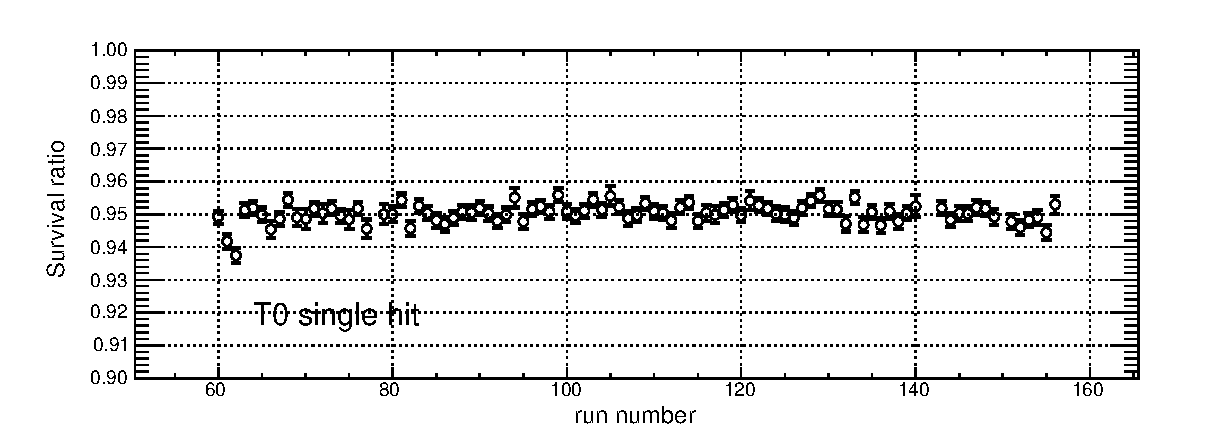
\includegraphics[width=\columnwidth]{./fig/rundep-t0single.eps}
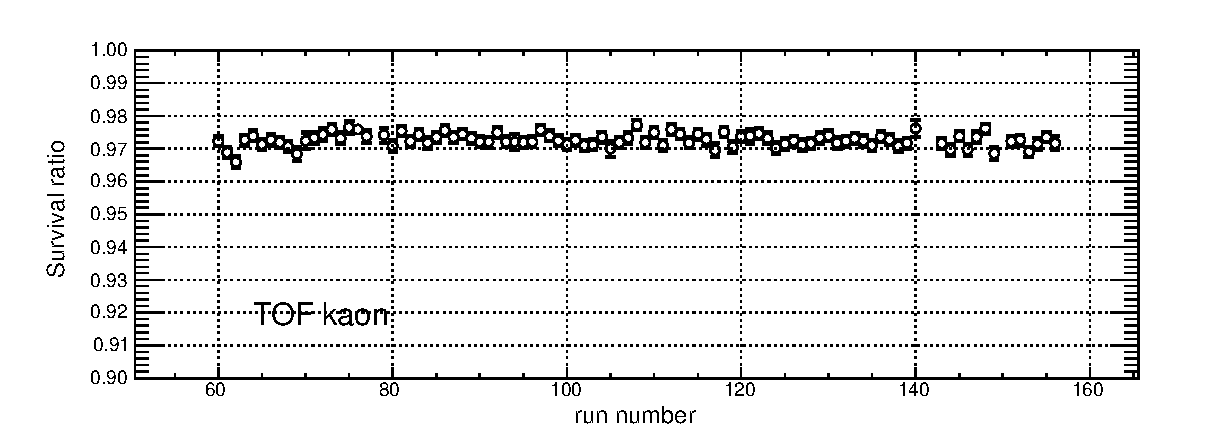
\includegraphics[width=\columnwidth]{./fig/rundep-tofk.eps}
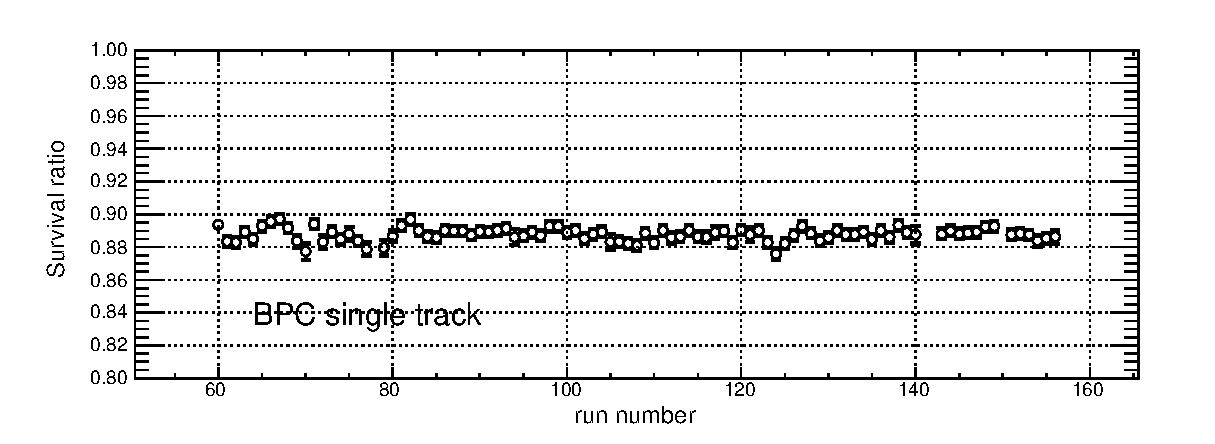
\includegraphics[width=\columnwidth]{./fig/rundep-bpcsingle.eps}
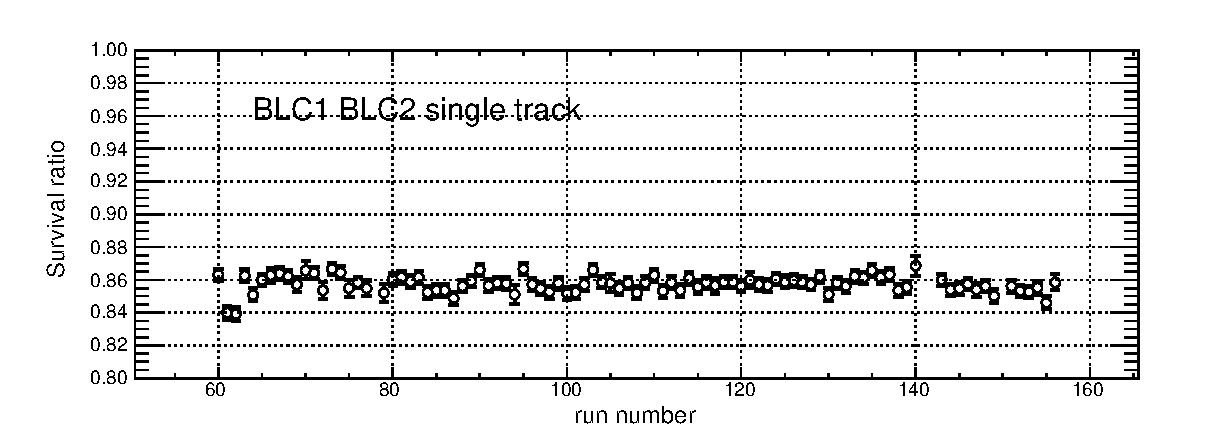
\includegraphics[width=\columnwidth]{./fig/rundep-blc12single.eps}
\caption{Run dependence}
%\label{fig-ncsimeff}
\end{center}
\end{figure}  

\begin{figure}[tbp]
\begin{center}
%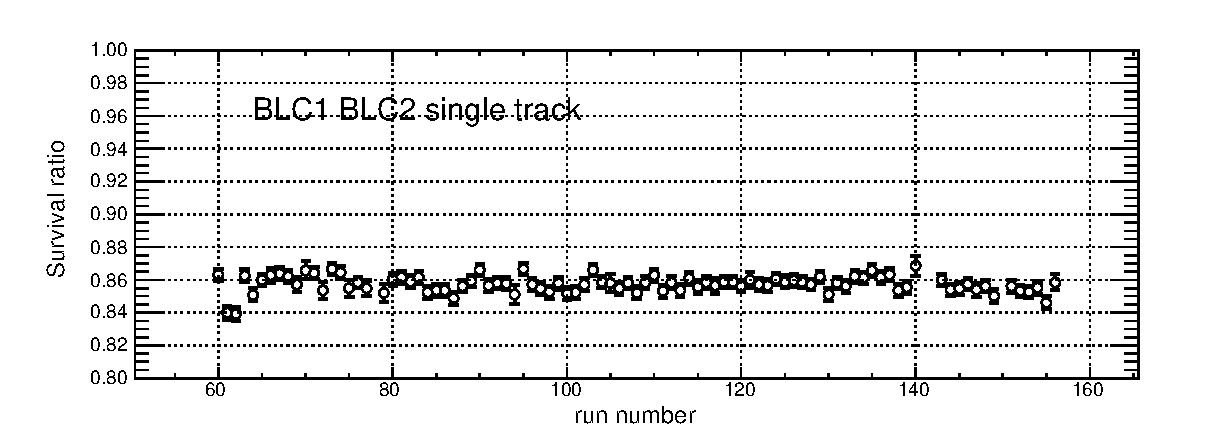
\includegraphics[width=\columnwidth]{./fig/rundep-blc12single.eps}
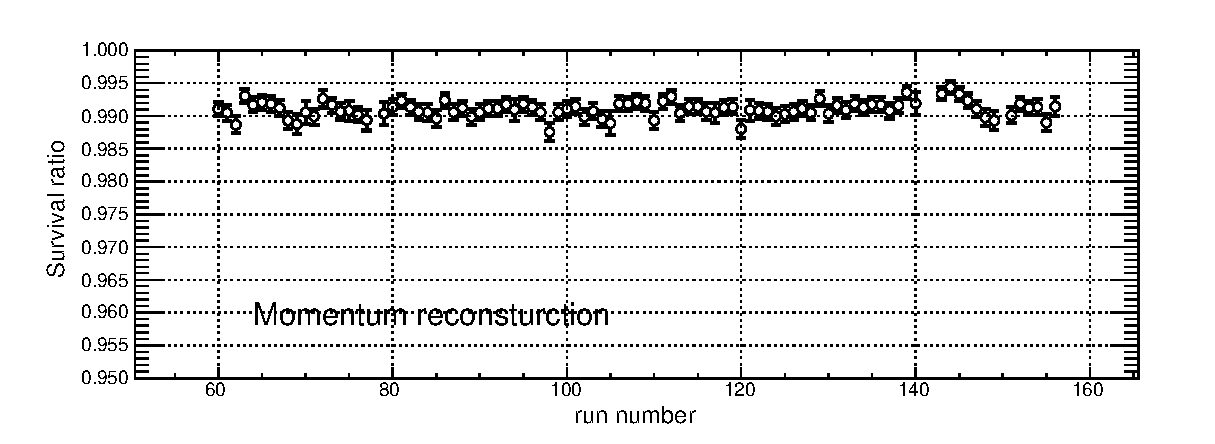
\includegraphics[width=\columnwidth]{./fig/rundep-mom.eps}
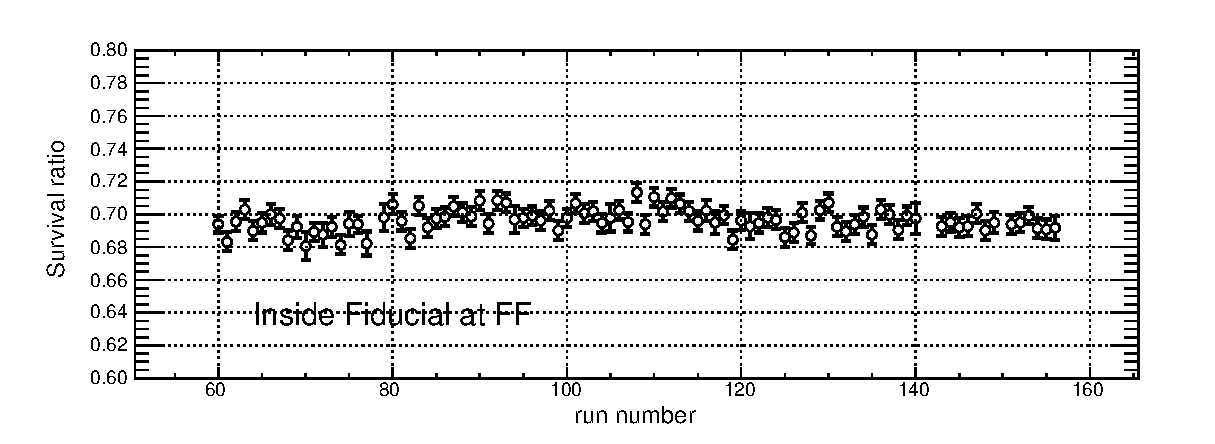
\includegraphics[width=\columnwidth]{./fig/rundep-fiducial.eps}
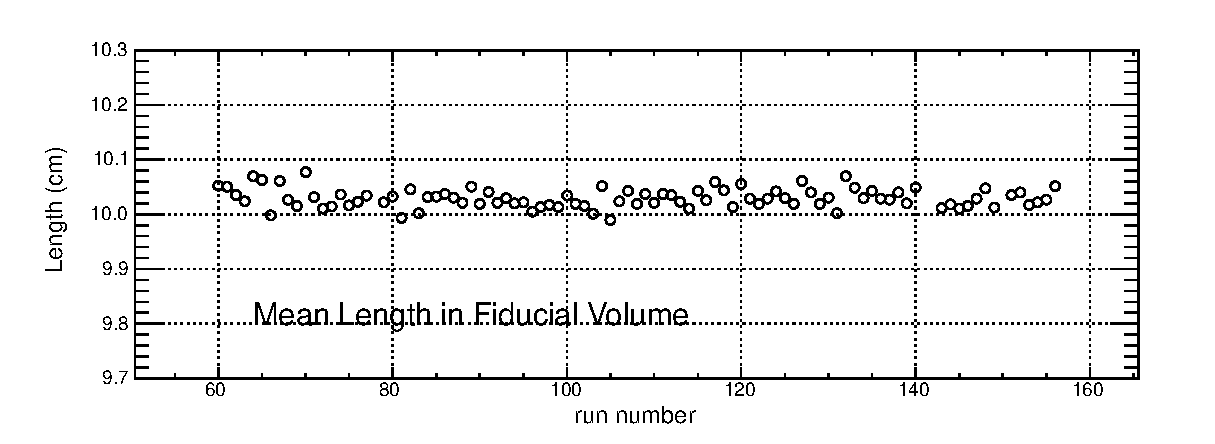
\includegraphics[width=\columnwidth]{./fig/rundep-length.eps}
\caption{Run dependence}
%\label{fig-ncsimeff}
\end{center}
\end{figure}  

\section{CDS performance}


\begin{figure}[tbp]
\begin{center}
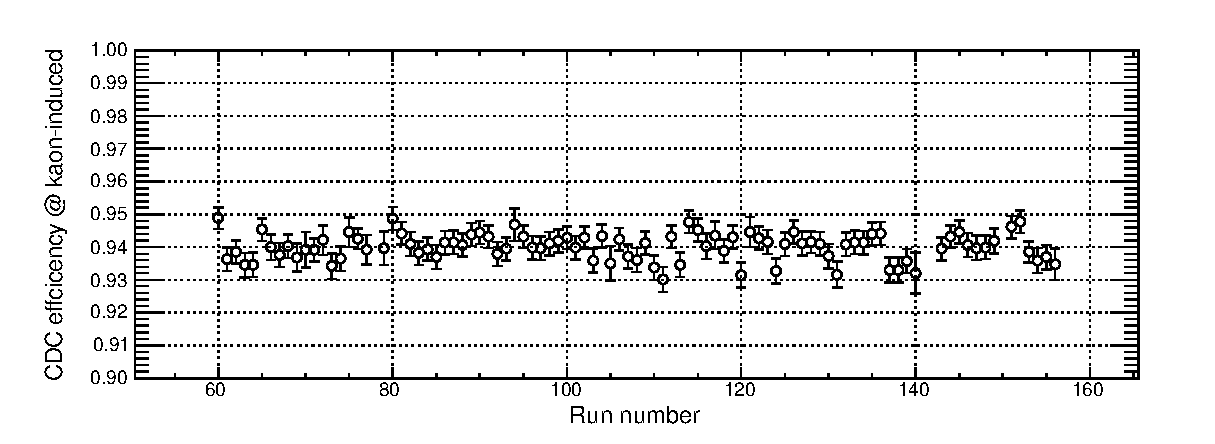
\includegraphics[width=\columnwidth]{./fig/rundep-cdceff.eps}
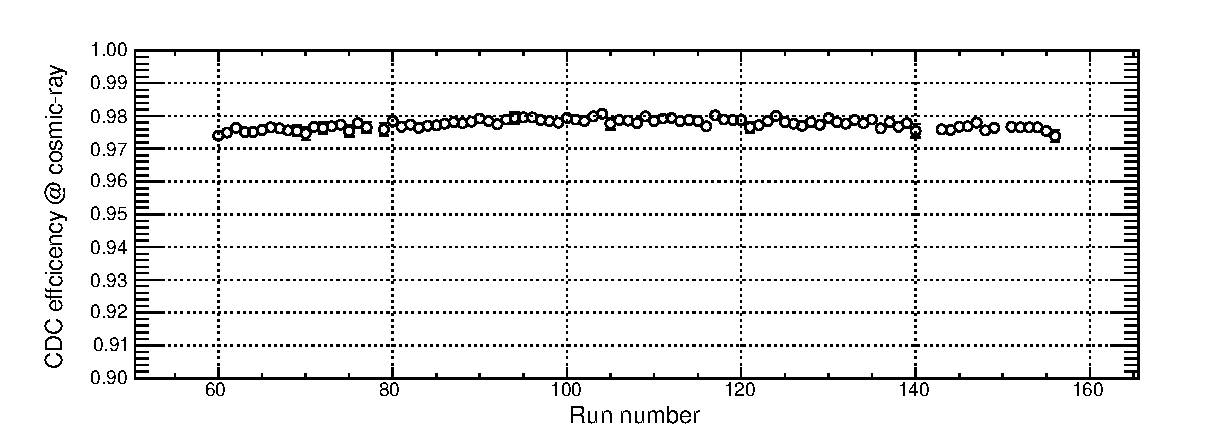
\includegraphics[width=\columnwidth]{./fig/rundep-cosmiceff.eps}
\caption{Run dependence}
%\label{fig-ncsimeff}
\end{center}
\end{figure}  

\begin{figure}[tbp]
\begin{center}
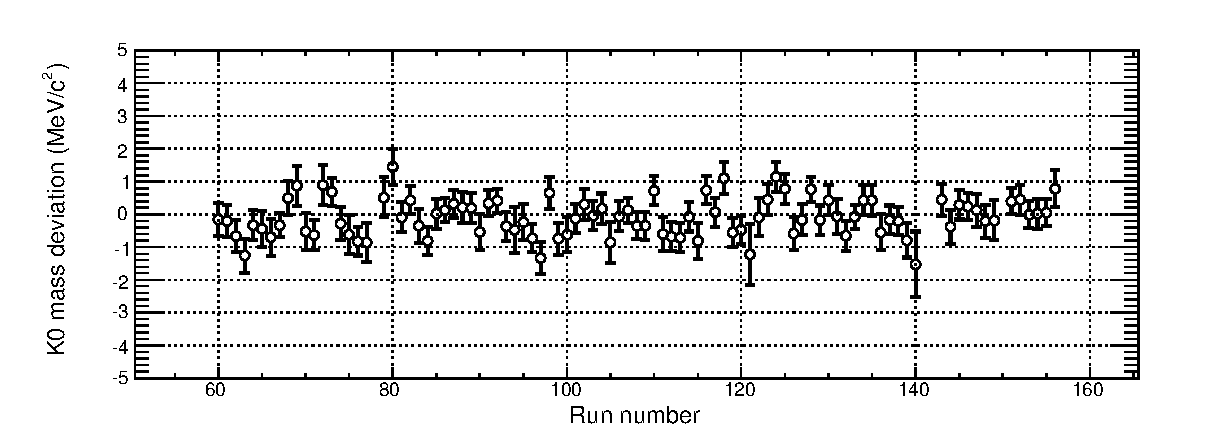
\includegraphics[width=\columnwidth]{./fig/rundep-k0mass.eps}
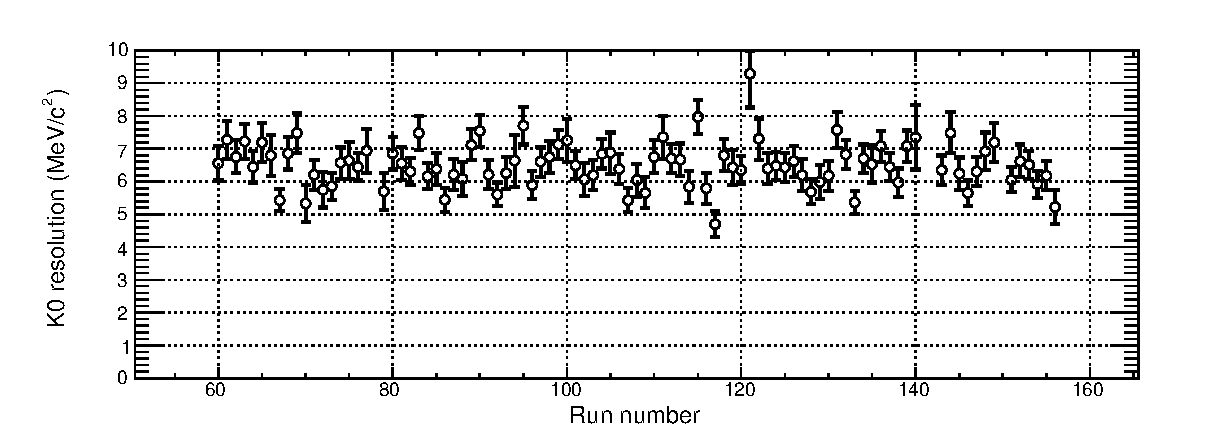
\includegraphics[width=\columnwidth]{./fig/rundep-k0res.eps}
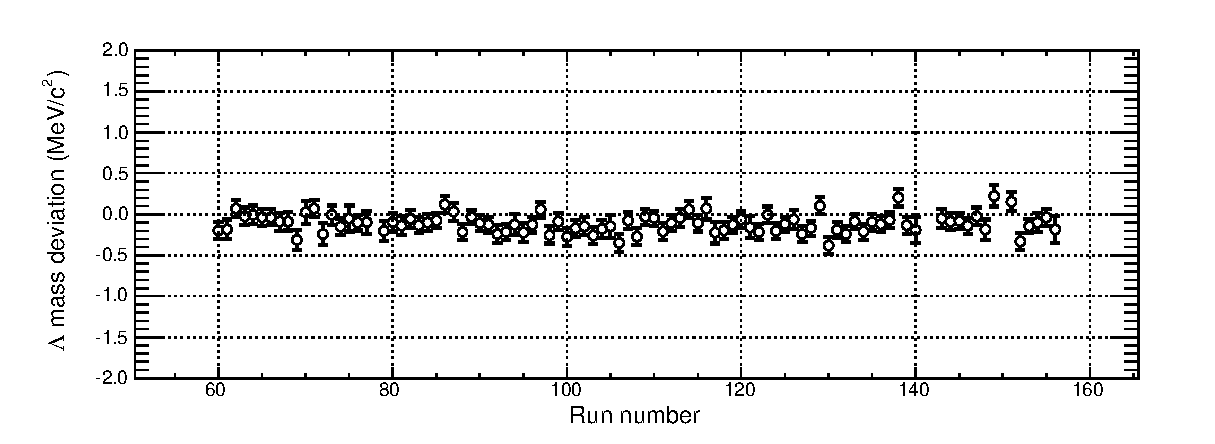
\includegraphics[width=\columnwidth]{./fig/rundep-lmass.eps}
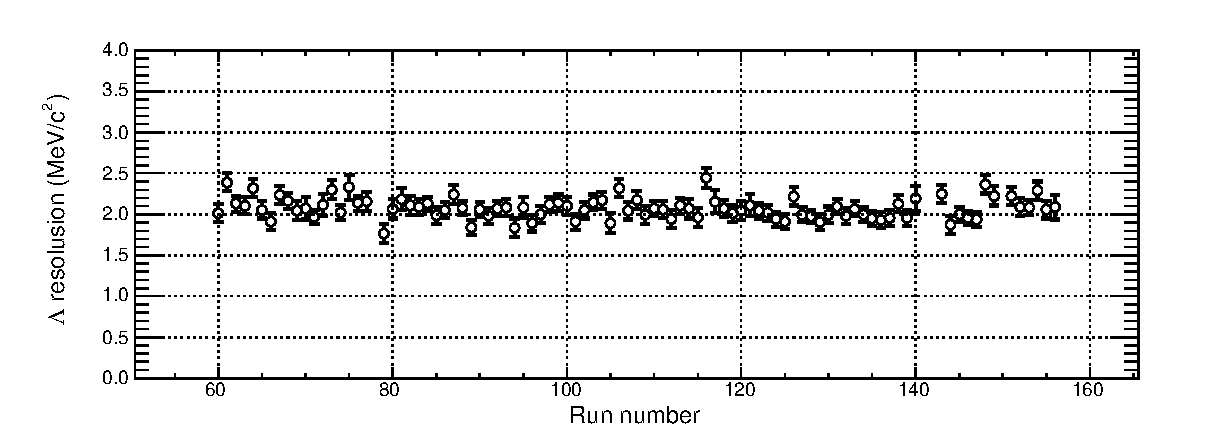
\includegraphics[width=\columnwidth]{./fig/rundep-lres.eps}
\caption{Run dependence}
%\label{fig-ncsimeff}
\end{center}
\end{figure}  

\section{Normalization factors}
\begin{figure}[tbp]
\begin{center}
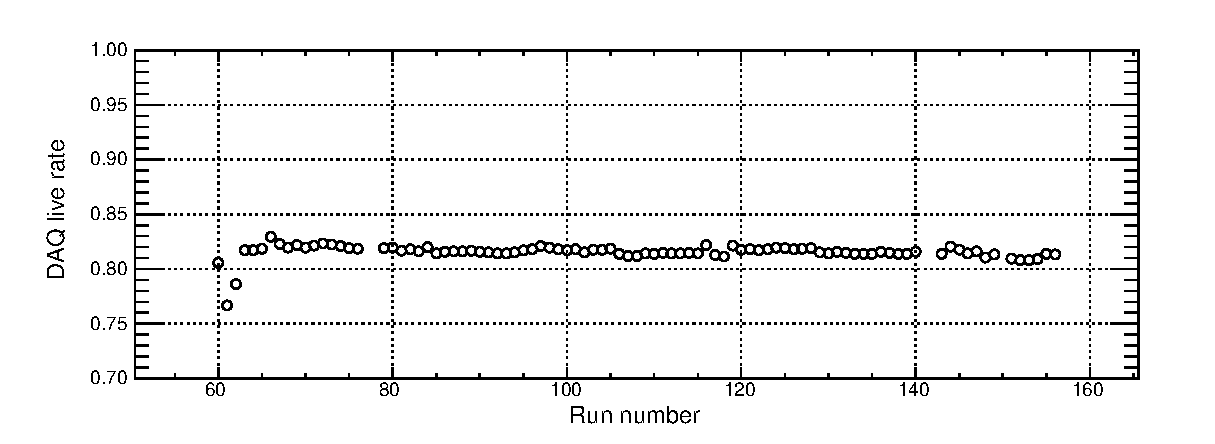
\includegraphics[width=\columnwidth]{./fig/rundep-daq.eps}
\caption{Run dependence}
%\label{fig-ncsimeff}
\end{center}
\end{figure}  


\end{document}
